\section{\texttt{bimodal}}\label{sec:bimodal_bimodal}


This example replicates the problem in ``Section 4.1 A 1D Problem'' of~\cite{CheungPrudencio2012}: it presents how to use QUESO and the multivevel method for sampling from a posterior PDF composed of the sum of two Gaussian distributions. 

Let's define $D=[-250,250]$ and the three distributions $\pi_\prior: D \rightarrow \mathbb{R}_+ $, $f_1: \mathbb{R} \rightarrow \mathbb{R}_+ $ and $f_2: \mathbb{R} \rightarrow \mathbb{R}_+$ by:
\begin{equation}
\begin{split}\label{eq:bimodal_functions}
\pi_\prior &=  \dfrac{1}{|D|} = \dfrac{1}{500}, \quad \forall \,  \theta \in D \\
f_1(\theta) &= \dfrac{1}{(2\pi)^{1/2} \sqrt{|V_1|}} \exp \left(-\dfrac{1}{2}(\theta - \mu_1)^T \, V_1^{-1} \, (\theta - \mu_1) \right), \quad \forall \,  \theta \in \mathbb{R} \\
f_2(\theta) &= \dfrac{1}{(2\pi)^{1/2} \sqrt{|V_2|}} \exp \left(-\dfrac{1}{2}(\theta - \mu_2)^T \, V_2^{-1} \, (\theta - \mu_2) \right), \quad \forall \, \theta \in \mathbb{R},
\end{split}
\end{equation}
where
\begin{equation*}
\mu_1 = 10, \quad  V_1 = 1^2, \quad \mu_2 = 100, \quad V_2= 5^2.
\end{equation*}

In this example, we want to sample the posterior PDF given by:
\begin{equation}
\pi_\post(\theta)  \propto \left[\dfrac{1}{2} f_1(\theta) + \dfrac{1}{2} f_2(\theta) \right] \cdot \pi_\prior = f(\theta) \cdot \pi_\prior
\end{equation}
where $f(\theta)= \dfrac{1}{2} f_1(\theta) + \dfrac{1}{2} f_2(\theta)$ is the likelihood function, which is depicted in Figure \ref{fig:bimodal:likelihood}.

\begin{figure}[htpb]
\centering
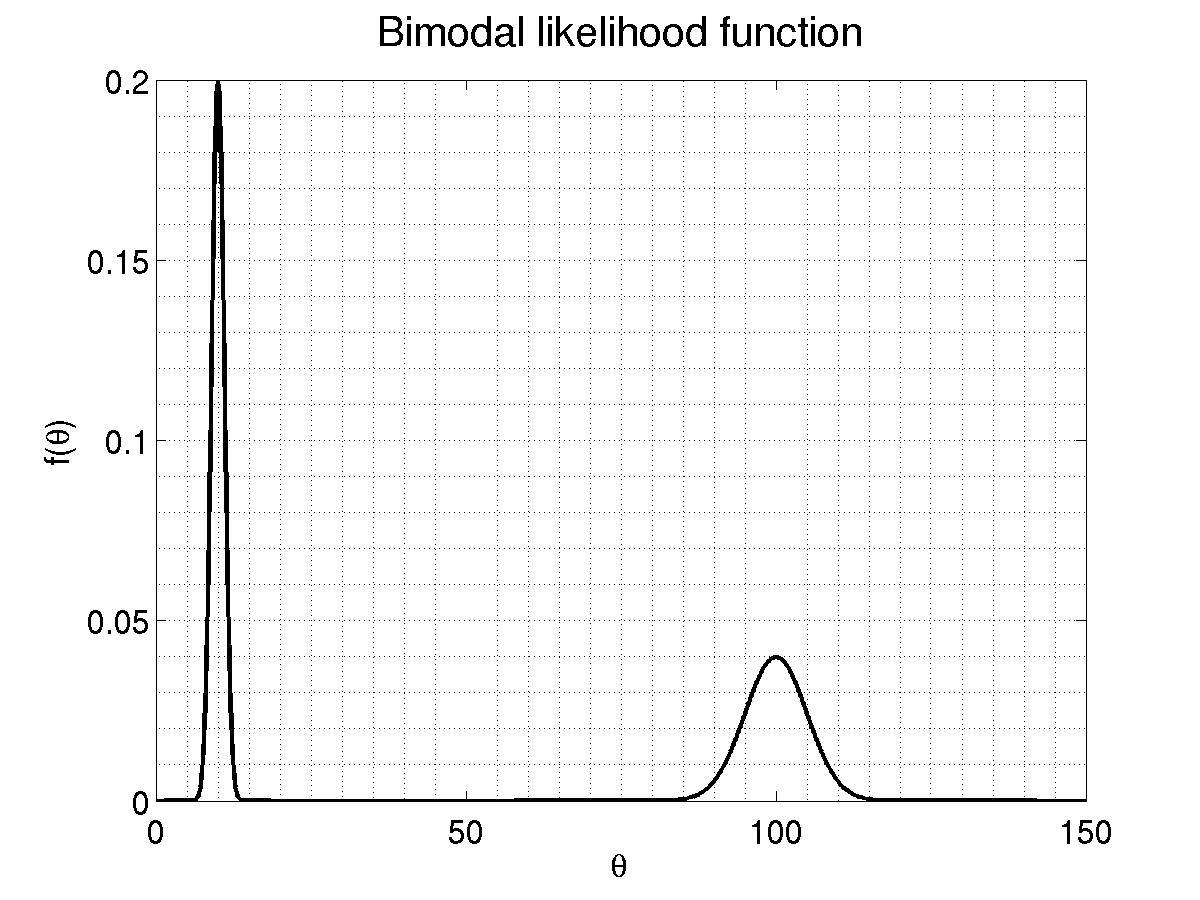
\includegraphics[scale=0.3]{figs/bimodal_likelihood.png}
\vspace{-10pt}
\caption{Likelihood function given by $f=f_1/2+ f_2/2$, where $f_1$ and $f_2$ are defined in Equation \eqref{eq:bimodal_functions}.}
\label{fig:bimodal:likelihood}
\end{figure}


\subsection{Running the Example}\label{sec:bimodal-run}

To run the executable provided (available after QUESO installation), and generate figures for the chains, PDFs, CDFs, etc., enter the following commands:
\begin{lstlisting}[label={},caption={}]
$ cd $HOME/LIBRARIES/QUESO-0.50.0/examples/bimodal
$ rm outputData/*
$ ./bimodal_gsl bimodal_1chain.inp    
$ matlab
   $ plot_all.m	                          # inside matlab
   $ plot_likelihood_normalized_taus.m    # inside matlab
   $ plot_likelihood_unnormalized_taus.m  # inside matlab
   $ exit                                 # inside matlab
$ ls -l outputData/*.png
bimodal_autocorrelation_rawchain.png  bimodal_likelihood.png
bimodal_cdf_rawchain.png	          bimodal_likelihood_taus_normalized.png
bimodal_kde_rawchain.png	          bimodal_likelihood_taus.png
\end{lstlisting}


As a result, the user should have created several of PNG figures containing marginal posterior PDF, cumulative density distribution and autocorrelation. The name of the figure files have been chosen to be informative, as shown in the Listing above.




\subsection{Example Code}\label{sec:bimodal-code}

The source code for the example is composed of 5 files:
\texttt{bimodal\_main.C} (Listing \ref{code:bimodal-main-c}), \linebreak
\texttt{bimodal\_likelihood.h} and \texttt{bimodal\_likelihood.C} (Listings \ref{fig-like-bimodal-h} and \ref{fig-like-bimodal-c}),
\texttt{bimodal\_compute.h} and \texttt{bimodal\_compute.C} (Listings \ref{code:bimodal-compute-h} and \ref{code:bimodal-compute-c}).


\lstinputlisting[caption=File \texttt{bimodal\_main.C.}, label={code:bimodal-main-c}, linerange={25-1000}]{../../examples/bimodal/src/bimodal_main.C}

\lstinputlisting[caption=File \texttt{bimodal\_likelihood.h}., label={fig-like-bimodal-h}, linerange={25-1000}]{../../examples/bimodal/src/bimodal_likelihood.h}

\lstinputlisting[caption=File \texttt{bimodal\_likelihood.C}., label={fig-like-bimodal-c}, linerange={25-1000}]{../../examples/bimodal/src/bimodal_likelihood.C}

\lstinputlisting[caption=File \texttt{bimodal\_compute.h.}, label={code:bimodal-compute-h}, linerange={25-1000}]{../../examples/bimodal/src/bimodal_compute.h}

Note that in line 57 of Listings \ref{code:bimodal-compute-c} the `\verb+#if 0+' directive tells the compiler that the application will not use DRAM algorithm, but rather the Multilevel solver (line 65). Naturally, the user may chose to use the DRAM algorithm by changing the directive in line 57 to `\verb+#if 1+'.

\lstinputlisting[caption={File \texttt{bimodal\_compute.C}.}, label={code:bimodal-compute-c}, linerange={25-1000},numbers=left]{../../examples/bimodal/src/bimodal_compute.C}
 
  


\subsection{Input File}\label{sec:bimodal-input-file}


QUESO reads an input file for solving statistical problems, which provides options for the Multilevel or MCMC method. In this example, the Multilevel method is chosen to sample from the distribution. Many variables are common to both MCMC and Multilevel method, especially because the Multilevel method also has the option of delaying the rejection of a candidate. The names of the variables have been designed to be informative in this case as well:
\begin{description}\vspace{-8pt}
\item[ \texttt{env}:] refers to QUESO environment; \vspace{-8pt}
\item[ \texttt{ip}:] refers to inverse problem;\vspace{-8pt}
\item[ \texttt{ml}:] refers to Multilevel;\vspace{-8pt}
\item[ \texttt{dr}:] refers to delayed rejection;\vspace{-8pt}
\item[ \texttt{rawChain}:] refers to the raw, entire chain; \vspace{-8pt}
\item[ \texttt{filteredChain}:] refers to a filtered chain (related to a specified \texttt{lag});\vspace{-8pt}
\item[ \texttt{last}:] refers to instructions specific for the last level of the Multilevel algorithm.
\end{description}

The user may select options for a specific level by naming its number, i.e., in case the user wants to define a different number of extra stages together with the scales for each stage (in the DRAM part of the ML algorithm) for the level 3, he/she may include the following instructions:
\begin{lstlisting}
ip_ml_3_dr_maxNumExtraStages          = 1
ip_ml_3_dr_listOfScalesForExtraStages = 3.333
\end{lstlisting}
in the input file.


The options used for solving this example are displayed in Listing \ref{code:bimodal-input-file}. 

\lstinputlisting[caption={Options for QUESO library used in application code (Listings \ref{code:bimodal-main-c}-\ref{code:bimodal-compute-c}})., 
label={code:bimodal-input-file},]{../../examples/bimodal/tests/test_2013_12_02/bimodal_1chain.inp}



\subsection{Create your own Makefile}\label{sec:bimodal-makefile}

Similarly to the other examples presented in this user's manual and also available with QUESO distribution, a user-created makefile is available: `\texttt{Makefile\_bimodal\_violeta}'. When adapted to the user's settings, namely paths for  QUESO required libraries, it may be used to compile the code and create the executable \verb+bimodal_gsl+. 

Thus, to compile, build and execute the code, the user just needs to run the following commands in the same directory where the files are:
\begin{lstlisting}
$ cd $HOME/LIBRARIES/QUESO-0.50.0/examples/bimodal/
$ export LD_LIBRARY_PATH=$LD_LIBRARY_PATH:\
  $HOME/LIBRARIES/gsl-1.15/lib/:\
  $HOME/LIBRARIES/boost-1.53.0/lib/:\
  $HOME/LIBRARIES/hdf5-1.8.10/lib:\
  $HOME/LIBRARIES/QUESO-0.50.0/lib 
$ make -f Makefile_bimodal_violeta 
$ ./bimodal_gsl example.inp
\end{lstlisting}

Again, the `\verb+export+' instruction above is only necessary if the user has not saved it in his/her \verb+.bashrc+ file. 


\subsection{Data Post-Processing and Visualization}\label{sec:bimodal-results}



According to the specifications of the input file in Listing~\ref{code:bimodal-input-file}, both a folder named \verb+outputData+ and a the following files should be generated:
\begin{verbatim}
rawChain_ml.m 
display_sub0.txt    
\end{verbatim}


The sequence of Matlab commands is identical to the ones presented in Sections
\ref{sec:sip-results}, \ref{sec:sfp-results}, \ref{sec:gravity-results} and \ref{sec:tga-results};
therefore, are omitted here. The reader is invited to explore the Matlab files
\texttt{plot\_likelihood\_normalized\_taus.m},
\texttt{plot\_likelihood\_unnormalized\_taus.m} and/or \texttt{plot\_all.m},  for details of how the figures have been generated.



\subsubsection{KDE and CDF Plots}

Figure \ref{fig:bimodal_kde} presents the KDE and CDF plots of the parameter $\theta$. 



\begin{figure}[hptb]
\centering
\subfloat[KDE]{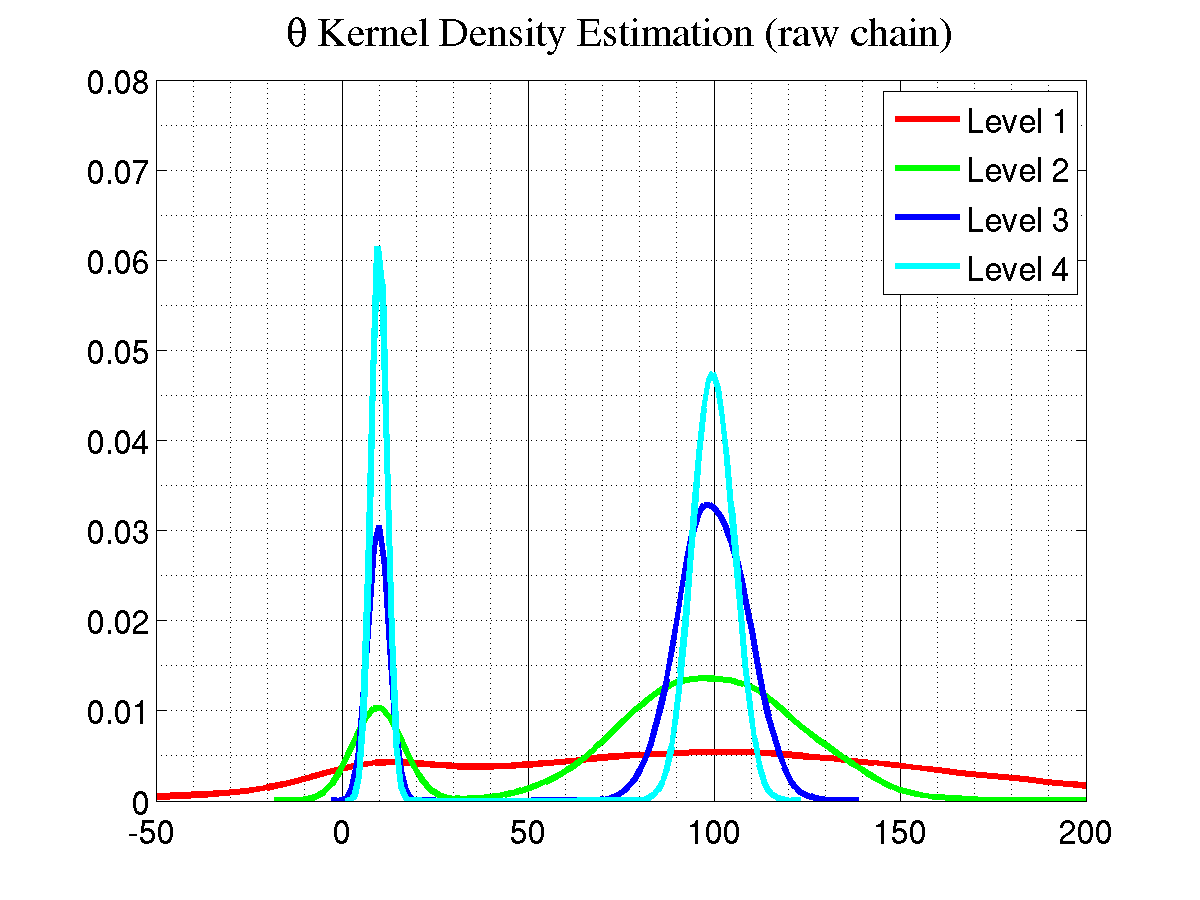
\includegraphics[scale=0.3]{figs/bimodal_kde_rawchain.png}}
\subfloat[CDF]{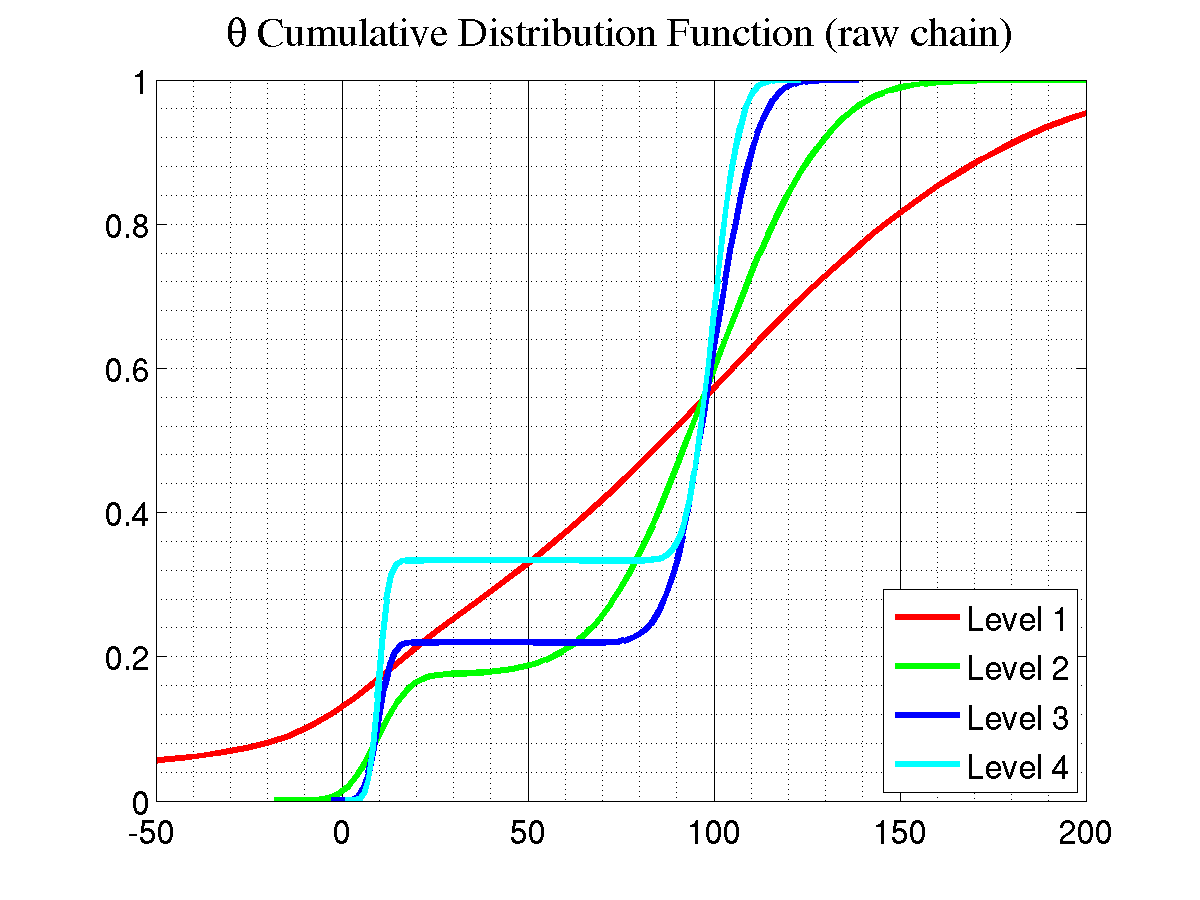
\includegraphics[scale=0.3]{figs/bimodal_cdf_rawchain.png}}
\vspace{-8pt}
\caption{KDE and CDF plots of parameter $\theta$, for all fours levels.}
\label{fig:bimodal_kde}
\end{figure}

\subsubsection{Autocorrelation Plots}

Figure \ref{fig:bimodal_autocorr} presents the autocorrelation of the parameter $\theta$, in each one of the intermediate levels.

\begin{figure}[htpb]
\centering
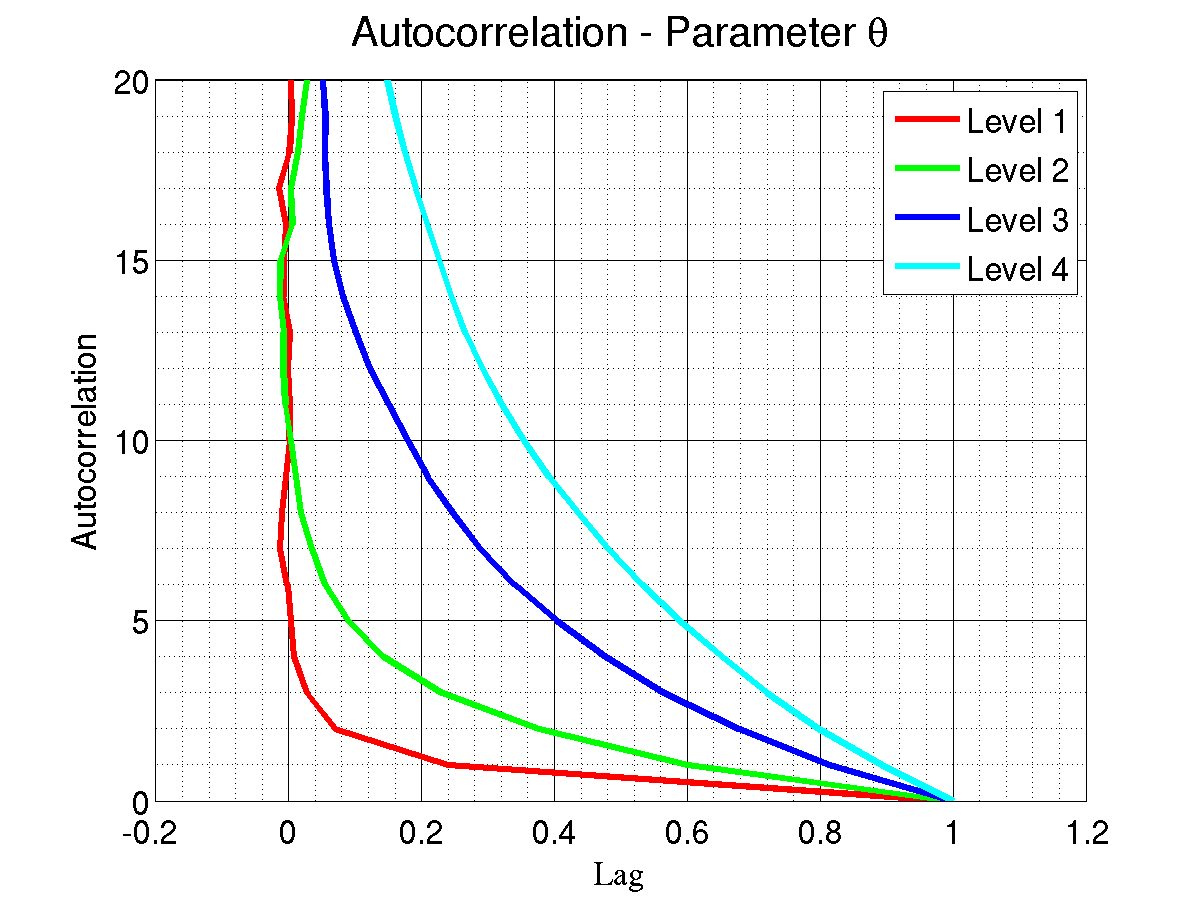
\includegraphics[scale=0.25]{figs/bimodal_autocorrelation_rawchain}
\vspace{-10pt}
\caption{Autocorrelation plots for $\theta$, all four levels.}
\label{fig:bimodal_autocorr}
\end{figure}



\subsubsection{Intermediary Likelihood Plots}
\begin{figure}[htpb]
\centering
\subfloat[normalized]{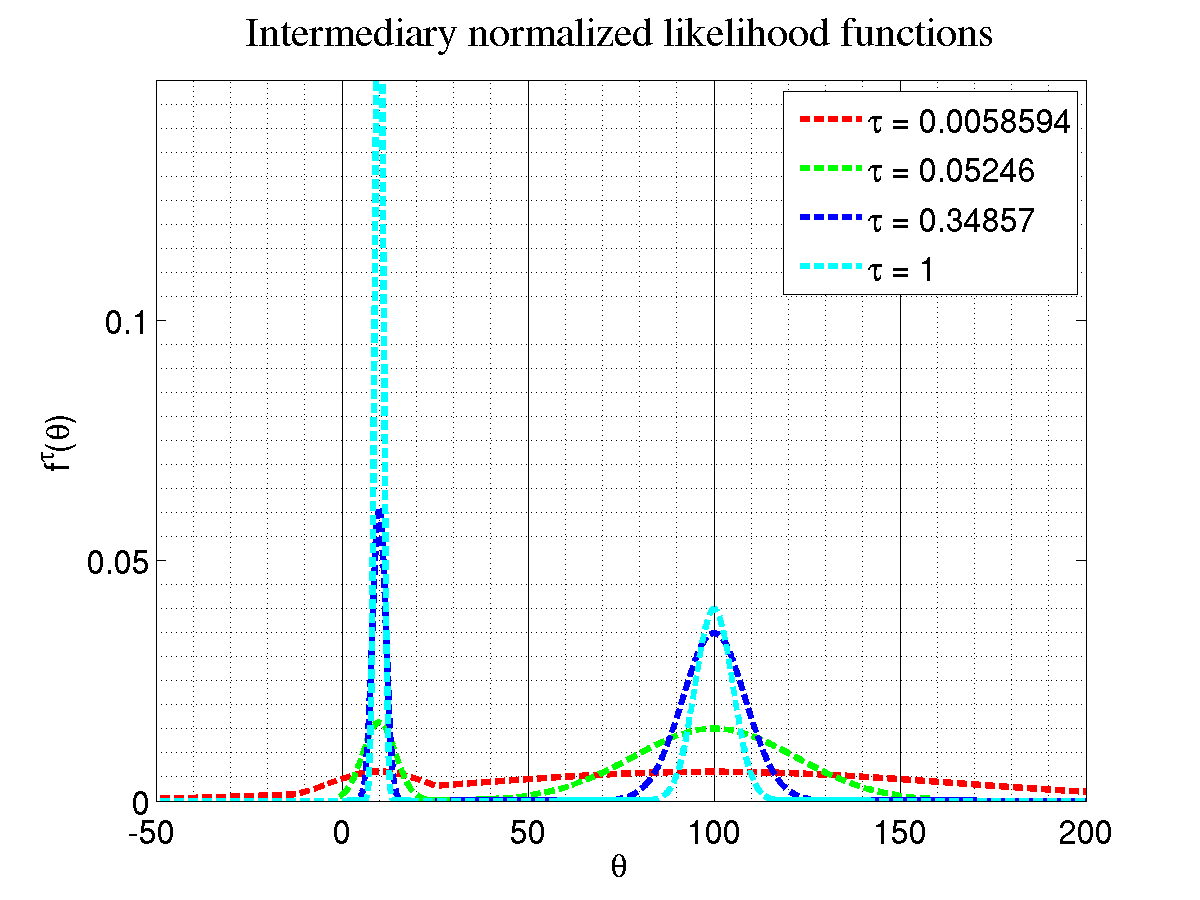
\includegraphics[scale=0.3]{figs/bimodal_likelihood_taus_normalized.png}}
\subfloat[unnormalized]{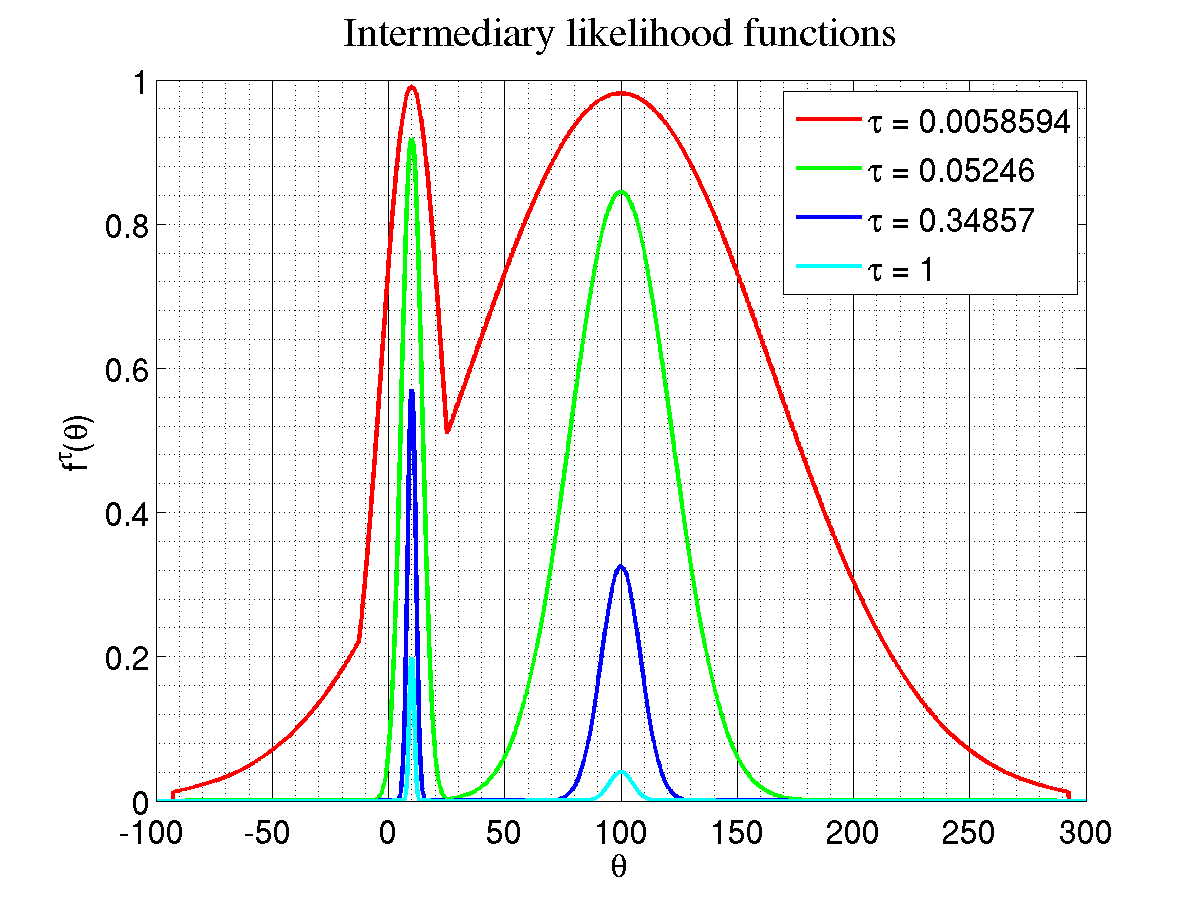
\includegraphics[scale=0.3]{figs/bimodal_likelihood_taus.png}}
\vspace{-10pt}
\caption{Intermediary likelihood functions $f(\theta)^\tau$, where $\tau_i$ is the exponent computed at the $i$-th level of Multilevel algorithm. In this simple problem, only four levels are needed, i.e. $i=1\ldots 4$. The cyan-colored curve (exponent $\tau = 1$) is the same curve as in Figure \ref{fig:bimodal:likelihood}.}
\label{fig:bimodal:likelihood_taus}
\end{figure}
